\documentclass{beamer}
\usepackage{graphicx}
\usepackage{listings}

\lstdefinestyle{basic}{showstringspaces=false,
                       columns=fullflexible,
                       language=C++,
                       escapechar=@,
                       basicstyle=\tiny\sffamily,
classoffset=1,
morekeywords={attr_level_set,spawn,wait}
keywordstyle=[1]\color{blue}, 
classoffset=0,
moredelim=**[is][\color{white}]{~}{~},
literate={->}{{$\rightarrow\;$}}1 {<-}{{$\leftarrow\;$}}1 {=>}{{$\Rightarrow\;$}}1,
}
\lstset{language=C++,style=basic}

\newenvironment{discuss}{\begin{list}{}{}\item[]{\it Discussion item:}
\addcontentsline{toc}{subsection}{Discussion Item}
}{{\rm ({\it End of discussion item.})} \end{list}}
\newcommand{\code}[1]{\lstinline[basicstyle=\sffamily]{#1}}
\newcommand{\func}[1]{\lstinline[basicstyle=\sffamily]{#1()}}
\newcommand{\Cpp}{C\kern-0.05em\texttt{+\kern-0.03em+}}
\newcommand{\MPIpp}{MPI\kern-0.05em\texttt{+\kern-0.03em+}}
\newcommand{\tablefont}{\fontsize{8}{13}\selectfont}
\newcommand{\halfline}{\vspace{-1.0ex}}

\mode<presentation>
{
  \usetheme{Warsaw}
  \setbeamercovered{transparent}
  \definecolor{TUCGreen}{RGB}{0,100,50}
  \definecolor{TUCGreenlight}{RGB}{120,200,150}
  \definecolor{IURed}{RGB}{255,0,0}
  \definecolor{IURedlight}{RGB}{255,204,204}
  \definecolor{OMPIBlue}{RGB}{80,130,255}
  \definecolor{OMPIBluelight}{RGB}{240,240,255}
  \definecolor{white}{RGB}{255,255,255}
  \definecolor{black}{RGB}{0,0,0}
  \setbeamercolor*{palette primary}{fg=white, bg=IURed}
  \setbeamercolor*{palette secondary}{fg=white, bg=IURed}
  \setbeamercolor*{palette tertiary}{fg=white, bg=IURed}
  \setbeamercolor*{palette quartenary}{fg=white, bg=IURed}
  \setbeamercolor*{palette sidebar primary}{fg=white, bg=IURed}
  \setbeamercolor*{palette sidebar secondary}{fg=white, bg=IURed}
  \setbeamercolor*{palette sidebar tertiary}{fg=white, bg=IURed}
  \setbeamercolor*{palette sidebar quartenary}{fg=white, bg=IURed}
  \setbeamercolor*{normal text}{fg=black, bg=white}
  \setbeamercolor*{example text}{fg=black, bg=white}
  \setbeamercolor*{titlelike}{fg=white, bg=IURed}
  \setbeamercolor*{separation line}{fg=white, bg=IURed}
  \setbeamercolor*{item projected}{fg=white, bg=IURed}
  \setbeamercolor*{block title}{fg=white, bg=IURed}
  \setbeamercolor*{block title alerted}{fg=IURed, bg=white}
  \setbeamercolor*{block title example}{fg=IURed, bg=white}
  \setbeamercolor{block body}{fg=black, bg=IURedlight}
  \setbeamercolor*{structure}{fg=IURed, bg=white}
  \setbeamercolor*{sidebar}{fg=IURed, bg=white}
  % or whatever (possibly just delete it)
}

\setbeamertemplate{background canvas}

\usepackage[english]{babel}
\usepackage[latin1]{inputenc}
\usepackage{times}
\usepackage[T1]{fontenc}

\title{PFunc: Modern Task Parallelism For Modern High Performance Computing}

\author{Prabhanjan Kambadur}

\date{{\small SC 2009}
{\footnotesize Portland, OR}\\
$19^{th}$ Nov 2009}

\begin{document}

\begin{frame}
  \titlepage
\end{frame}

\begin{frame}
\frametitle{Motivation.}
\begin{itemize}
\item Parallelize a wide-variety of applications.
  \begin{itemize}
  \item Traditional HPC, informatics and mainstream.
  \end{itemize}
\item Parallelize for modern architectures.
  \begin{itemize}
  \item Multi-core, many-core and GPGPUs.
  \end{itemize}
\item Enable user-driven optimizations.
  \begin{itemize}
  \item Fine-tune application performance.
  \item No runtime penalties.
  \end{itemize}
\item Mix SPMD-style programming with tasks.
\end{itemize}
\end{frame}

\begin{frame}
\frametitle{PFunc: Key features.}
\begin{itemize}
\item Extends existing task parallel feature-set. 
  \begin{itemize}
  \item Cilk, Threading Building Blocks, Fortran M, etc.
  \end{itemize}
\item Portable.
  \begin{itemize}
  \item Linux, OS X, AIX and \textcolor{gray}{Windows}.
  \end{itemize}
\item Customizable.
  \begin{itemize}
  \item Generic and generative programming techniques.
  \item No runtime penalty for customizations.
  \end{itemize}
\item C and \Cpp{} APIs.
\end{itemize}
\end{frame}

\begin{frame}[fragile]
\frametitle{Overview of PFunc}

\tablefont
\begin{center}
\textcolor{blue}{Most aspects of PFunc are customizable, with suitable defaults!}
\end{center}

\begin{center}
\tablefont
\begin{tabular}{|c|l|}
\hline
\textcolor{blue}{Feature} & Explanation \\
\hline
\textcolor{blue}{Scheduling Policy} & $\ast{}$ Determines task scheduling. \\
          & $\ast{}$ Default values can be used (eg., \textcolor{blue}{cilkS}). \\
\hline
\textcolor{blue}{Compare} & $\ast{}$ Ordering function for task priorities. \\
      & $\ast{}$ \textcolor{blue}{Priority}, an inherited feature can also be customized. \\
\hline
\textcolor{blue}{Functor} & $\ast{}$ Type of the parallel function. \\
                          & $\ast{}$ In some situations, avoids virtual function costs. \\
\hline
\end{tabular}
\end{center}

\normalsize

\begin{center}
\begin{minipage}{0.6\textwidth}
\begin{lstlisting}
struct fibonacci;
typedef pfunc::generator<cilkS, /* scheduling policy */
                         use_default, /* compare */
                         fibonacci> my_pfunc; /*function object*/
\end{lstlisting}
\end{minipage}
\end{center}

\end{frame}

\begin{frame}[fragile]
\frametitle{Important types.}
\begin{center}
\tablefont
\begin{tabular}{|c|l|}
\hline
\textcolor{blue}{Type} & Explanation \\
\hline
\textcolor{blue}{Attribute} & $\ast{}$ Attached to each task. \\
          & $\ast{}$ Priority, affinity, group affiliation, etc \\
          & $\ast{}$ Default values can be used (eg., Fibonacci). \\
\hline
\textcolor{blue}{Group} & $\ast{}$ Used for SPMD-style programming. \\
      & $\ast{}$ Point-to-point, barrier operations. \\
      & $\ast{}$ Default values can be used (eg., Fibonacci). \\
\hline
\textcolor{blue}{Task} & $\ast{}$ Handle to a spawned ``\textcolor{red}{task}''. \\
     & $\ast{}$ Used for status inspection. \\
\hline
\textcolor{blue}{TaskMgr} & $\ast{}$ An instance of PFunc's runtime. \\
        & $\ast{}$ Encapsulates threads, task queues and scheduling policy. \\
        & $\ast{}$ Multiple taskmgr's can exist simultaneously. \\
\hline
\end{tabular}
\end{center}

\normalsize

\begin{center}
\begin{minipage}{0.5\textwidth}
\begin{lstlisting}
typedef my_pfunc::attribute my_attribute; /* attribute */
typedef my_pfunc::group  my_group; /* group */
typedef my_pfunc::task my_task; /* task handle */
typedef my_pfunc::taskmgr my_taskmgr; /* runtime */
typedef my_pfunc::functor my_functor; /* type of functor */
\end{lstlisting}
\end{minipage}
\end{center}

\end{frame}

\begin{frame}[fragile]
\frametitle{Fibonacci numbers.}
\begin{center}
\begin{minipage}{0.60\textwidth}
\begin{lstlisting}
my_taskmgr *gbl_taskmgr; /* Initialized in main() */
@\halfline@
struct fibonacci {
  private:
  const int n;
  int fib_n;
@\halfline@
  public:
  fibonacci (const int& n) : n(n), fib_n(0) {}
@\halfline@
  int get_number () const { return fib_n; }
@\halfline@
  void operator () (void) {
@\halfline@
    if (0 == n || 1 == n) fib_n = n;
    else {
      task tsk; 
      attribute nested_attr;
@\halfline@
      fibonacci fib_n_1 (n-1);
      fibonacci fib_n_2 (n-2);
@\halfline@
      pfunc::attr_level_set (nested_attr, (0xFFFFFFFF-(n-1)));
      pfunc::spawn (*gbl_taskmgr, tsk, nested_attr, fib_n_1);
@\halfline@
      fib_n_2();
@\halfline@
      pfunc::wait (*gbl_taskmgr, tsk);
@\halfline@
      fib_n = fib_n_1.get_number () + fib_n_2.get_number ();
    }
  }
};
\end{lstlisting}
\end{minipage}
\end{center}
\end{frame}

\begin{frame}[fragile]
\frametitle{Fibonacci: task creation overhead.}
$\rightarrow{}$ \textcolor{blue}{Fibonacci number 37 ($2^{36}\approx{}69$ billion tasks).}
\tablefont
\begin{center}
\begin{tabular}{|c|c|c|c|c|} 
\hline
Threads & Cilk Time (secs) & PFunc/Cilk & TBB/Cilk & PFunc/TBB \\
\hline
1  & 2.17 & 2.2178  & 4.431 & 0.5004 \\ 
\hline
2  & 1.15 & 2.1135 & 4.1924 & 0.5041 \\ 
\hline
4  & 0.55 & 2.2131 & 4.4183 & 0.5009 \\ 
\hline
8  & 0.28 & 2.2114 & 4.9839 & 0.4437 \\ 
\hline
16 & 0.15 & 2.4944 & 5.9370 & 0.4201 \\ 
\hline
\end{tabular}
\end{center}
\normalsize
\begin{itemize}
\item \textcolor{red}{2x faster than TBB!}
\item Only 2x slower than Cilk.
  \begin{itemize}
  \item \textcolor{red}{But provides more flexibility!}
    \begin{itemize}
    \item Fibonacci is the \textcolor{red}{worst} case behavior.
    \end{itemize}
  \item Library-based rather than a custom compiler.
  \end{itemize}
\end{itemize}
\tiny\textcolor{blue}{$\ast{}$4 socket, quad-core AMD 8356 with Linux 2.6.24.}\normalsize
\end{frame}

\begin{frame}[fragile]
\frametitle{New features.}
\begin{itemize}
\item Customizable task scheduling and priorities.
\begin{center}
\tablefont
\begin{tabular}{|c|l|l|}
\hline
\textcolor{blue}{Sched policy} & Explanation & Task priority \\
\hline
\textcolor{blue}{cilkS} & Cilk-style scheduling & Not used \\
\hline
\textcolor{blue}{prioS} & Priority-based scheduling & \textcolor{red}{Used} \\
\hline
\textcolor{blue}{proxS} & Proximity-based scheduling using k-d tree & \textcolor{red}{Used} \\
\hline
\textcolor{blue}{fifoS} & Queue-based scheduling & Not used \\
\hline
\textcolor{blue}{lifoS} & Stack-based scheduling & Not used \\
\hline
\end{tabular}
\normalsize
\end{center}
  \begin{itemize}
  \item \textcolor{blue}{Informatics and real-time applications.}
  \end{itemize}
\item Multiple completion notifications.
  \begin{itemize}
  \item Tasks can return to \textcolor{red}{multiple} parents/\textcolor{red}{siblings}.
  \item \textcolor{blue}{Natural parallelization of DAG executions}.
  \end{itemize}
\end{itemize}
\end{frame}

\begin{frame}
\frametitle{New features.}
\begin{itemize}
\item Task groups.
  \begin{itemize}
  \item SPMD-style parallelization.
    \begin{itemize}
    \item Point-to-point and barrier operations.
    \end{itemize}
  \item \textcolor{blue}{Iterative sparse solvers.}
  \end{itemize}
\item Task affinities.
  \begin{itemize}
  \item Heterogeneous computer architectures.
  \item Attach tasks to queues and queues to processors.
  \item \textcolor{blue}{Optimize for NUMA and GPGPU machines.}
  \end{itemize}
\item Exception handling.
  \begin{itemize}
  \item Exceptions delivered to \textcolor{red}{spawn} sites.
  \end{itemize}
\item Performance profiling.
  \begin{itemize}
  \item PAPI integration.
  \end{itemize}
\end{itemize}
\end{frame}

\begin{frame}[fragile]
\frametitle{Case studies}
\framesubtitle{Demand-driven DAG execution}
\begin{itemize}
\item Data-driven execution of DAGs has many shortcomings.
  \begin{itemize}
  \item Increased memory consumption in many applications.
  \item Over-parallelization $\rightarrow{}$ \textcolor{blue}{Sparse Cholesky Factorization}.
  \end{itemize}
\item Current solutions support demand-driven tree execution.
  \begin{itemize}
  \item DAGs can be executed only using data-driven model.
  \item Side-effect of using \textcolor{blue}{strict} computational model.
  \end{itemize}
\item PFunc allows demand-driven execution of DAGs.
  \begin{itemize}
  \item Multiple task completion notifications.
  \item Task priorities to control execution.
  \end{itemize}
\end{itemize}
\end{frame}

\begin{frame}[fragile]
\frametitle{Results}
\framesubtitle{Multiple completion notifications: DAG execution (runtime).}
\begin{figure}
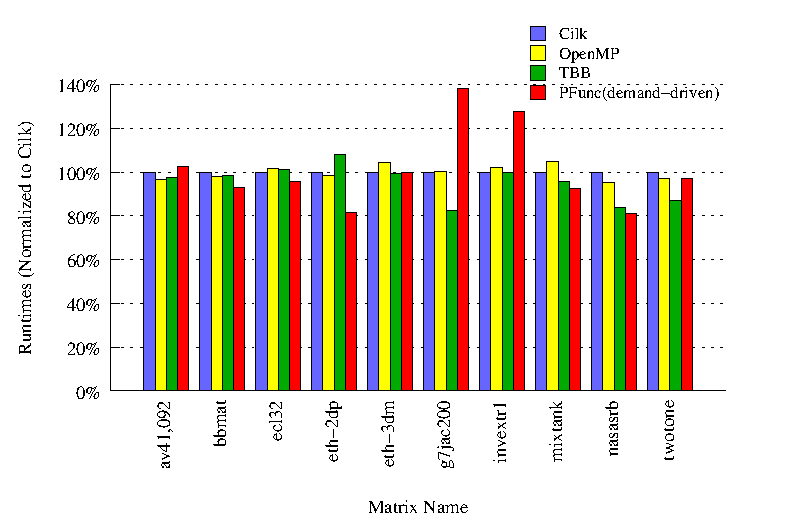
\includegraphics[width=0.9\textwidth]{figs/dag_speedup}
\label{fig:dag_speedup}
\end{figure}
\end{frame}

\begin{frame}[fragile]
\frametitle{Results}
\framesubtitle{Multiple completion notifications: DAG execution (peak memory).}
\begin{figure}
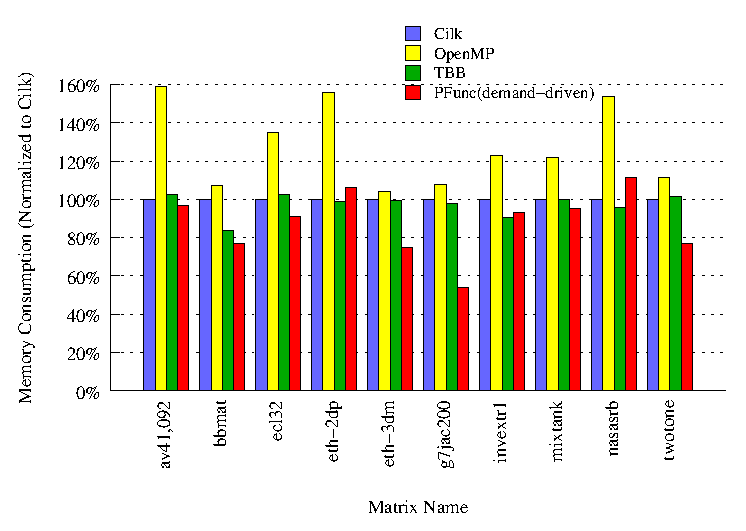
\includegraphics[width=0.9\textwidth]{figs/dag_memory}
\label{fig:dag_memory}
\end{figure}
\end{frame}

\begin{frame}[fragile]
\frametitle{Case studies}
\framesubtitle{Frequent Pattern Mining}
\begin{itemize}
\item Frequent pattern mining applications are not recursive!
  \begin{itemize}
  \item The best algorithms are breadth-first (eg., Apriori).
  \item Optimal execution $\rightarrow{}$ memory reuse b/w tasks.
  \end{itemize}
\item Current solutions do not support custom task affinities.
  \begin{itemize}
  \item Affinities exploited in tree structured depth-first executions.
    \begin{itemize}
    \item Emphasis is on \textcolor{blue}{recursive} parallelism.
    \end{itemize}
  \item Task priorities are not supported.
  \end{itemize}
\item PFunc allows custom scheduling policies and priorities.
  \begin{itemize}
  \item Hash-tables used for task scheduling queues.
  \item Task priorities double as keys for individual tasks.
  \end{itemize}
\end{itemize}
\end{frame}

\begin{frame}[fragile]
\frametitle{Results}
\framesubtitle{Custom task scheduling and priority: frequent pattern mining.}
\begin{figure}
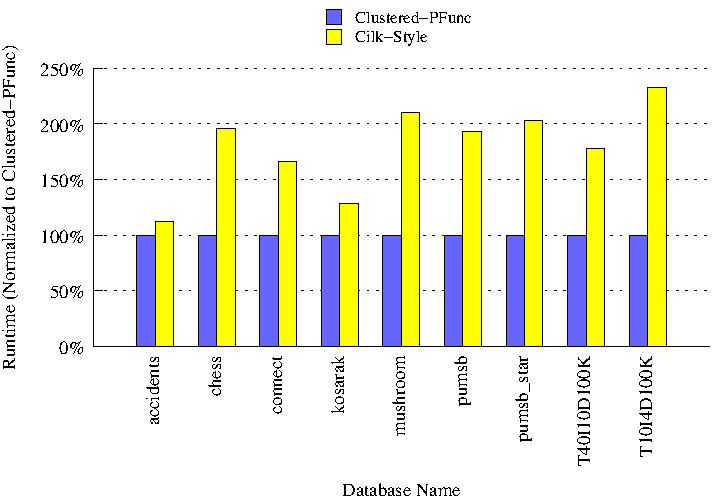
\includegraphics[width=0.8\textwidth]{figs/fim_8}
\label{fig:fim}
\end{figure}
\end{frame}

\begin{frame}[fragile]
\frametitle{Case studies}
\framesubtitle{Iterative sparse solvers}
\begin{itemize}
\item Efficient parallelization requires
  \begin{itemize}
  \item SPMD $\rightarrow{}$ unpreconditioned iterative sparse solvers.
  \item Task parallel $\rightarrow{}$ preconditioners.
    \begin{itemize}
    \item Incomplete factorization methods.
    \end{itemize}
  \end{itemize}
  \item Krylov-subspace iterative algorithms (CG, GMRES).
\item Current solutions do not support the SPMD model.
\item PFunc supports SPMD model through task groups.
  \begin{itemize}
  \item \textcolor{gray}{Point-to-point} and collective operations.
  \item \textcolor{gray}{Group cancellation}.
  \end{itemize}
\end{itemize}
\end{frame}

\begin{frame}[fragile]
\frametitle{Results}
\framesubtitle{Task groups: iterative sparse solvers.}
\begin{figure}
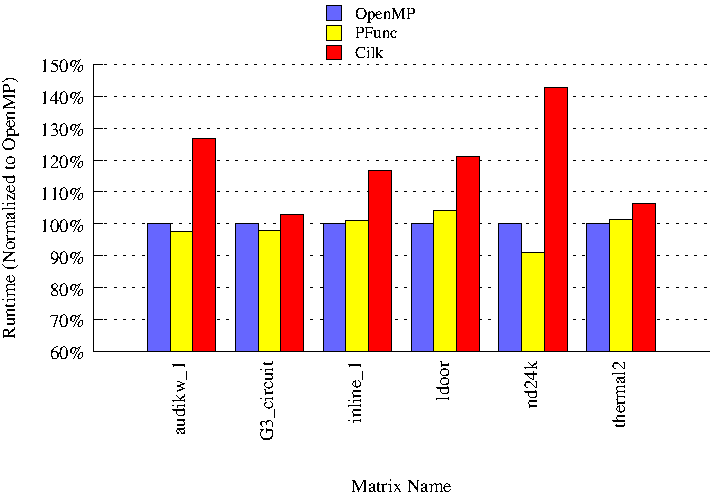
\includegraphics[width=0.9\textwidth]{figs/cg_8}
\label{fig:cg}
\end{figure}
\end{frame}

\begin{frame}
\frametitle{Conclusions}
\begin{itemize}
\item PFunc increases support for:
  \begin{itemize}
  \item Modern HPC applications.
  \item Modern computer architectures.
  \item SPMD-style programming.
  \item \textcolor{blue}{DAG execution, frequent pattern mining, sparse CG.}
  \end{itemize}
\item Future work.
  \begin{itemize}
  \item \textcolor{red}{Parallelize more applications!}
  \item Increase support for GPGPUs.
  \end{itemize}
\end{itemize}
\vspace{+10pt}
\begin{center}
\textcolor{blue}{$\ast{}$ https://projects.coin-or.org/PFunc $\ast{}$}
\end{center}
\end{frame}

\end{document}
